\documentclass[12pt]{report}
\usepackage[utf8]{inputenc}
\usepackage[portuguese]{babel}

\usepackage{graphicx}
\usepackage{tabularx}
\usepackage[section]{placeins}
\usepackage{hyperref}
\usepackage{xspace}

\usepackage{geometry}
\geometry{a4paper, total={150mm,225mm}, left=30mm, top=30mm}
\pagenumbering{arabic}

\usepackage[dvipsnames]{xcolor}
\usepackage{xargs}
\usepackage[colorinlistoftodos,prependcaption,textsize=tiny]{todonotes}
\newcommandx{\todonew}[2][1=]{\todo[linecolor=red,backgroundcolor=red!25,bordercolor=red,#1]{#2}}
\newcommandx{\todochange}[2][1=]{\todo[linecolor=orange,backgroundcolor=orange!25,bordercolor=orange,#1]{#2}}
\newcommandx{\todoreview}[2][1=]{\todo[linecolor=yellow,backgroundcolor=yellow!25,bordercolor=yellow,#1]{#2}}
\newcommandx{\todoimprove}[2][1=]{\todo[linecolor=green,backgroundcolor=green!25,bordercolor=green,#1]{#2}}
\newcommandx{\thiswillnotshow}[2][1=]{\todo[disable,#1]{#2}}

\begin{document}

\newcommand{\sajas}{\texttt{SAJaS}\xspace}
\newcommand{\jade}{\texttt{JADE}\xspace}
\newcommand{\repast}{\texttt{Repast 3}\xspace}
\newcommand{\massim}{\texttt{MASSim2Dev}\xspace}
\newcommand{\java}{\texttt{JAVA}\xspace}
\newcommand{\acl}{\texttt{ACL}\xspace}
\newcommand{\fipa}{\texttt{FIPA}\xspace}
\newcommand{\spotter}{\emph{spotter}\xspace}
\newcommand{\Spotter}{\emph{Spotter}\xspace}
\newcommand{\spotters}{\emph{spotters}\xspace}
\newcommand{\Spotters}{\emph{Spotters}\xspace}
\newcommand{\Producer}{\emph{Producer}\xspace}
\newcommand{\producer}{\emph{producer}\xspace}
\newcommand{\producers}{\emph{producers}\xspace}
\newcommand{\Producers}{\emph{Producers}\xspace}
\newcommand{\Transporter}{\emph{Transporter}\xspace}
\newcommand{\transporter}{\emph{transporter}\xspace}
\newcommand{\transporters}{\emph{transporters}\xspace}
\newcommand{\Transporters}{\emph{Transporters}\xspace}
\newcommand{\size}{\emph{size}\xspace}
\newcommand{\minerals}{\emph{minerals}\xspace}

\begin{titlepage}
	\begin{center}
		\vspace*{1cm}
        \Huge
        \textbf{Exploração de Marte}
        \vspace{0.5cm} \ \\
        \LARGE
        Agentes e Inteligência Artificial Distribuída
        \vfill
		
\includegraphics[width=0.6\textwidth]{FEUP_Logo}
		\break
        \small
        Dezembro 2016
        \vfill
		\vspace{1.5cm}
        \normalsize{
		\textbf{Grupo T05\_4} \\
		Marina Camilo - up201307722 - up201307722@fe.up.pt \\
		Diogo Ferreira - up201502853 - diogoff@fe.up.pt \\
		Ângela Cardoso - up200204375 - angela.cardoso@fe.up.pt
        }
	\end{center}
\end{titlepage}

\tableofcontents


%%%%%%%%%%%%%
% OBJECTIVO %
%%%%%%%%%%%%%
\chapter{Objetivo}

\section{Descrição do cenário}
No âmbito da unidade curricular de Agentes e Inteligência Artificial Distribuída, o nosso grupo propôs-se a implementar um Sistema Multi-Agente para simulação de um cenário de extração de minérios em Marte. Para tal, é necessário descobrir os minérios, extraí-los e transportá-los para a base. Sendo assim, no sistema pretendido existem três tipos de Agentes:

\begin{itemize}
	\item \Spotter – Procura fontes de minérios e inspeciona-as para determinar se podem ser exploradas. 
	\item \Producer – É chamado a uma fonte de minério por um \spotter para extrair o máximo de minério possível nessa fonte. 
	\item \Transporter – É alocado pelo \producer para carregar o minério obtido para a base.
\end{itemize}

De forma a facilitar a procura, todos os agentes podem localizar fontes de minérios e enviar a sua localização para os \spotters que os analisarão. A escolha do \producer por parte do \spotter segue um protocolo de negociação. A alocação dos \transporters a uma determinada fonte segue também um protocolo de negociação, iniciado pelo \producer. Esta alocação, terá em conta a quantidade de minério a transportar, de modo a determinar mais corretamente o número necessário de \transporters.

\section{Objetivos do trabalho}

Um dos objetivos deste trabalho é implementar os agentes de forma a que a simulação da exploração seja tão eficiente quanto possível. 

O nosso principal objetivo é utilizar este projeto como forma de melhor interiorizar os conceitos dos Sistemas Multi-Agente, nomeadamente ganhando uma maior familiaridade com as plataformas que permitem implementar e simular estes sistemas.


%%%%%%%%%%%%%%%%%
% ESPECIFICACAO %
%%%%%%%%%%%%%%%%%
\chapter{Especificação}

\section{Identificação e caracterização dos agentes}

\todoreview[inline]{arquitetura, comportamento, estratégias}
\todonew[inline]{processos de raciocínio - novo no relatório final}

Tal como descrito acima, o nosso sistema tem três tipos de agentes. De seguida descrevem-se mais detalhadamente estes agentes e a forma como os implementámos.

\subsection{\Spotter}
Cada \spotter tem a sua região conexa do espaço para explorar. Uma vez definida essa região, a estratégia do \Spotter é simples, encaminha-se para o inicio da região e inspeciona cada célula consecutivamente, determinando se contém minério extraível ou não e guarda registo desta informação. Sempre que encontra minério extraível, entra em contacto com todos os \producers para negociar e decidir qual deles será chamado para extrair o minério.

\subsection{\Producer}
Os \producers entram em ação assim que é encontrado minério extraível por um \spotter. Nesse momento cada um deles terá que determinar o custo necessário para se deslocar ao local e extrair o minério. Esse esforço corresponde à distância (em passos) a que o \producer se encontra do local no final de completar todas as tarefas em mãos, mais o tempo (em passos) que ele demorará a terminar a sua tarefa atual, caso esteja a extrair minério, mais o tempo que demorarão todas as outras tarefas com as quais já se tenha comprometido. Para esse efeito, cada \producer deve guardar uma fila contendo informação sobre as suas extrações, em particular o tempo que cada uma delas demora, incluindo a deslocação da sua posição anterior até ao local da extração.

\subsection{\Transporter}
Os \transporters iniciam a sua atividade quando são contactados para transportar minério. À semelhança do que acontece com os \producers, nesse momento terão de calcular o esforço que necessitam para se deslocarem ao local tendo em conta a sua capacidade final. Quando informarem os \producers do esforço que necessita para chegar até um local terá que considerar qual a capacidade que terá disponível quando lá se deslocar. O \producer escolhe os primeiros \transporters que totalizam a capacidade disponível da carga que se pretende transportar, regressando à base apenas quando atingem a carga máxima. 

\section{Protocolos de interação}

Existem 3 fases que se destacam no decorrer da simulação: repartição do espaço entre os \emph{spotters} existentes, requerimento de um \emph{producer} no momento de descoberta de um minério e, finalmente,
o escalonamento dos \emph{transporters} para a recolha dos fragmentos resultantes de um minério.

\todonew[inline]{incluir diagramas de interação UML, se aplicável}

\subsection{Divisão de espaços}
No inicio da simulação a nave-mãe divide o espaço disponível em linhas de acordo com o número de \emph{spotters} existentes e entrega cada um dos dados dos sub-espaços a um \spotter distinto de modo a que
este o possa depois confirmar com os restantes \emph{spotters} que pode realmente ficar responsável pela área. A Figura~\ref{space-sharing} demonstra como a nave-mãe faz esta divisão.

\begin{figure}[h]
	\centering
	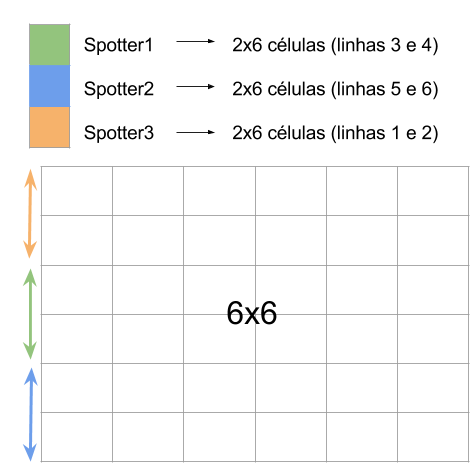
\includegraphics[width=0.4\textwidth]{space-sharing}
	\caption{Repartição de espaços}
	\label{space-sharing}
\end{figure}

Uma vez recebida a sugestão pela nave-mãe o \spotter inicia então o protocolo de negociação \textbf{fipa-propose} (Figura~\ref{fipa-propose}) com os restantes \emph{spotters}. Este protocolo define como propôr algo a outros agentes e
tratar das suas respostas.

\begin{figure}[h]
	\centering
	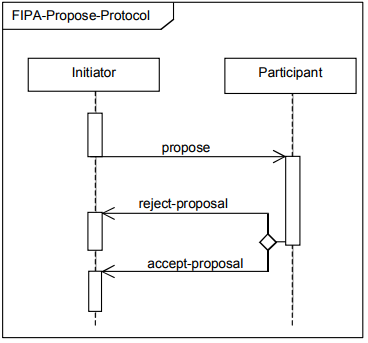
\includegraphics[width=0.4\textwidth]{fipa-propose}
	\caption{Repartição de espaços}
	\label{fipa-propose}
\end{figure}

Após a receção de todas as respostas é enviada uma última mensagem de volta a informar que a área ficou então afeta ao \spotter que iniciou a proposta. Esta última fase é complementar ao protocolo.
O protocolo \textbf{fipa-propose} é suportado pelas interfaces \emph{ProposeInitiator} e \emph{ProposeResponder} que um \spotter implementa através de \emph{behaviours} e pelas classes internas 
\emph{RequestAreaBehaviour} e \emph{AnswerCallBehaviour}, respetivamente.
Finalmente, a receção da última mensagem de notificação é feita também através de um \emph{behaviour} na classe interna \emph{AcknowledgeAreaBehaviour}. A mensagem tem a performativa \textbf{inform} e
no seu conteúdo uma string no formato \textbf{offset-height} em que \emph{offset} indica a coordenada no eixo Y em que a área começa e \emph{height} a altura da mesma. Os receptores desta mensagem
guardam então internamente num mapa esta afetação para possíveis futuras propostas.

\FloatBarrier
\subsection{Afetação de \producers}
Uma vez encontrado minério é necessário chamar um \producer para o extrair. O \spotter envia então a posição do  minério a todos os \producers. 
Estes respondem com o valor do esforço de que necessitarão para se deslocar até ao local. 
O \spotter escolhe o \producer com o menor esforço e comunica com ele, pedindo para confirmar a afetação. 
Caso seja recusado, porque o \producer foi afeto a outro minério entretanto, o \spotter repete o processo desde o início.

\begin{figure}[h]
	\centering
    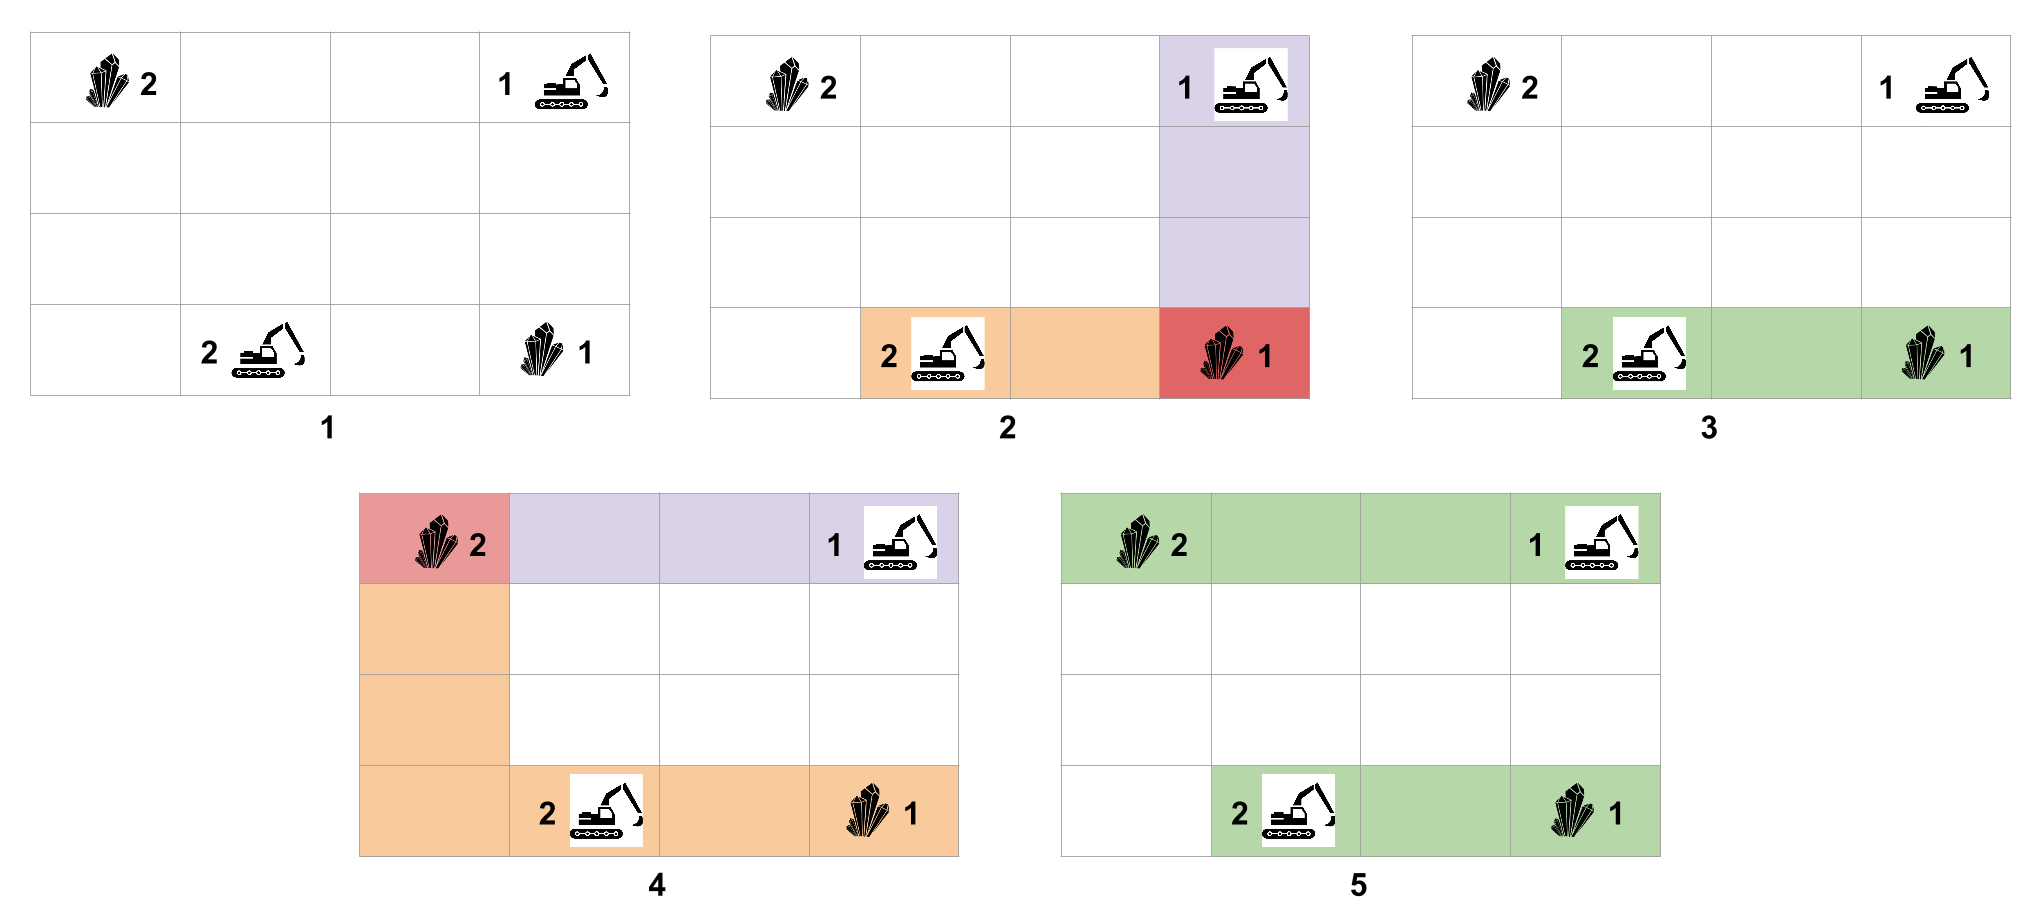
\includegraphics[width=0.8\textwidth]{producer-scheduling}
	\caption{Exemplo de afetação de \producers}
	\label{producer-scheduling}
\end{figure}

A Figura~\ref{producer-scheduling} exemplifica o processo de escolha de \producers para os minérios encontrados pelos \spotters 1 e 2. 
Neste caso, ficou o \producer 2 afeto ao minério do \spotter 1 e o \producer 1 afeto ao minério do \spotter 2.

\FloatBarrier
\subsection{Afetação de \transporters}
Após a extração do minério é necessário transportá-lo para a nave-mãe. 
O \producer que acabou de extrair o minério tem que selecionar um \transporter, do mesmo modo que o \spotter seleciona um \producer. 
Cada \transporter comunica o valor do esforço e o minério que consegue transportar possibilitando o \producer de escalonar os diferentes agentes.

\begin{figure}[h]
	\centering
    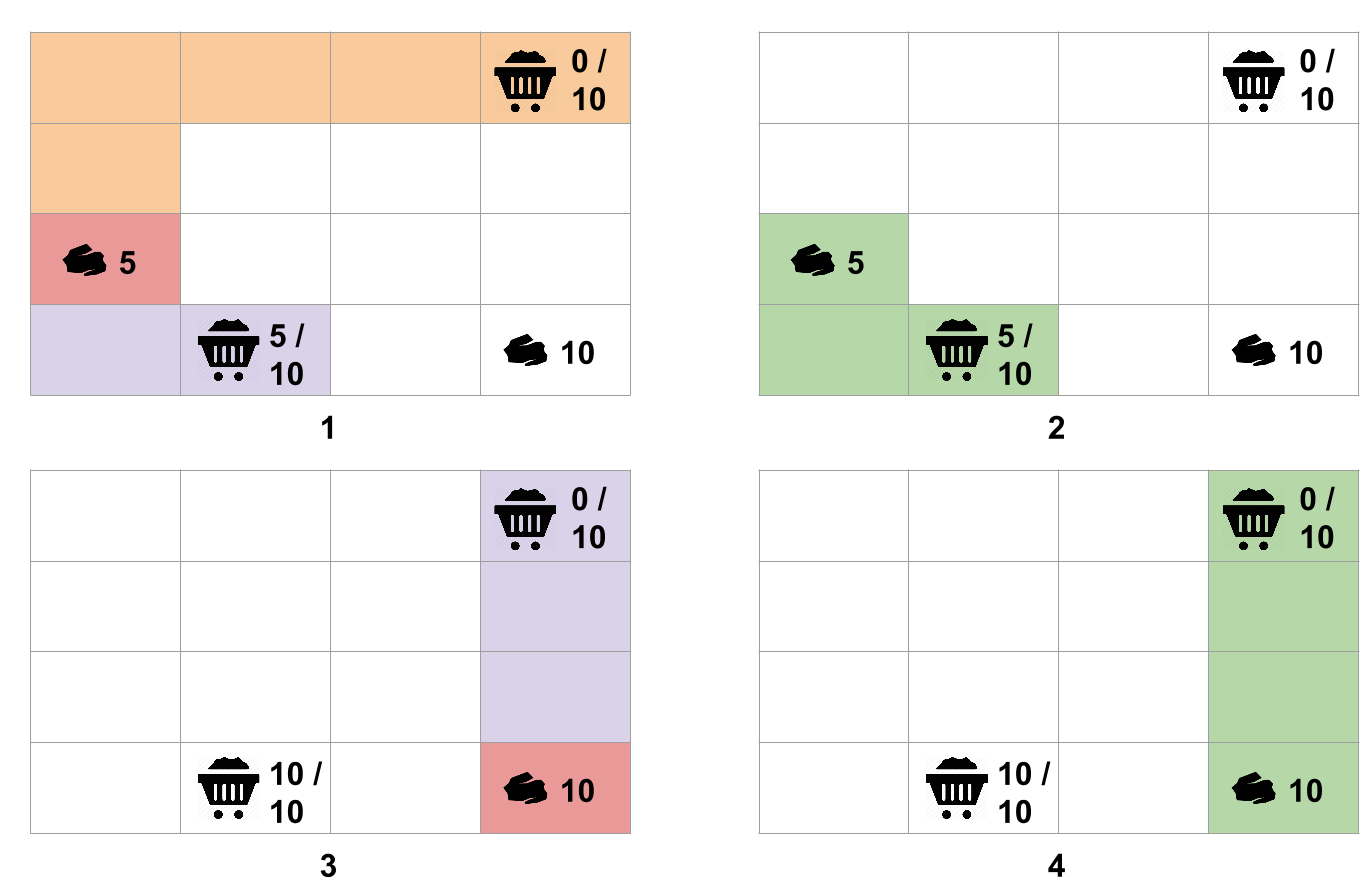
\includegraphics[width=0.8\textwidth]{transporter-scheduling}
	\caption{Exemplo de afetação de \transporters}
	\label{transporter-scheduling}
\end{figure}

A Figura~\ref{transporter-scheduling} exemplifica o processo de escolha de \transporters para os minérios extraídos por dois \producers. Consideramos ainda as quantidades de minério extraídas, a capacidade e carga corrente dos \transporters. Estas restrições irão influenciar a forma como se negoceia a afetação dos \transporters numa fase mais avançada da implementação.


%%%%%%%%%%%%%%%%%%%
% DESENVOLVIMENTO %
%%%%%%%%%%%%%%%%%%%
\chapter{Desenvolvimento}

\todonew[inline]{capítulo novo mas as secções não são completamente novas}

\section{Plataformas utilizadas}

\todoimprove[inline]{brevíssima descrição o que é - é capaz de ser melhor reduzir isto}

\subsection{\jade}
O \jade, \emph{Java Agent DEvelopment Framework}, é um software que permite desenvolver sistemas baseados em agentes. Os agentes são distribuídos por \emph{containers} que podem estar em máquinas diferentes, cada um utiliza uma \emph{thread}. 

O \jade é uma ferramenta totalmente escrita em \java, que suporta troca de mensagens \acl, seguindo a especificação \fipa. Além disso, possui um sistema de gestão de agentes e um sistema de páginas amarelas. Como os agentes estão distribuídos por contentores que podem estar em máquinas diferentes, permite ter agentes remotos. Os agentes podem migrar entre contentores e ser clonados. Esta plataforma possui ainda uma série de ferramentas que simplificam a administração e o desenvolvimento de aplicações, tais como:
\begin{itemize}
   \item agente de monitorização remota - interface gráfico para monitorizar a atividade dos agentes;
   \item agente pateta - permite trocar mensagens com outros agentes;
   \item agente inspetor - permite inspecionar outros agentes;
   \item agente introspetivo - permite monitorizar o ciclo de vida de um agente.
\end{itemize}

A implementação de agentes em \jade é feita recorrendo a comportamentos, que determinam as tarefas a executar pelos agentes consoante o contexto. 

\subsection{\repast}
O \repast, \emph{Recursive Porous Agent Simulation Toolkit}, é uma ferramenta de simulação baseada em agentes, que permite construir simulações locais à máquina com diversos agentes. O processamento de cada agente é distribuído por \emph{threads}.

O \repast suporta simulação de espaços físicos, representação 2D e 3D e análise em tempo real. Possui uma barra de ferramentas para controlar as simulações, um interface gráfico para manipular os parâmetros. Permite recolher dados em vários formatos, incluindo vários tipos de gráficos. A interação entre os agentes pode ser visualizada graficamente. Os espaços físicos simulados podem ser de variados tipos, como por exemplo, grelhas hexagonais ou retangulares, espaços contínuos ou redes. Além de poderem ser corridas com recurso ao interface gráfico, as simulações podem também ser lançadas em \emph{batch}.
  
O simulador discreto considera unidades de tempo - \emph{ticks} ou passos. Os eventos são planeados para ocorrer em \emph{ticks} específicos e assim é respeitada a ordem dos acontecimentos. Uma simulação considera um conjunto de agentes, cujos comportamentos são controlados recorrendo ao plano.

\subsection{\sajas}
O \sajas, \emph{Simple API for JADE-based Simulations}, é uma ferramenta que se propõe servir de ponte entre o desenvolvimento e a simulação de Sistemas Multi-Agente. Desta forma, através do \sajas, podemos tomar vantagem dos benefícios do \jade e do \repast.

O \sajas permite construir um Sistema Multi-Agente tal como é feito em \jade, existindo até uma ferramenta (\massim) que traduz código \jade para \sajas (e vice-versa), alterando as classes importadas. Ao contrário do \jade, permite ainda, recorrendo para isso ao \repast, a simulação deste tipo de sistemas. Além disso, o \sajas permite obter melhores performances do que numa simulação construída em \jade, que teria que considerar algum tipo de agente representado o `mundo'.

\subsection{Realce das funcionalidades relevantes para o trabalho}

Com o suporte do \jade são feitos os protocolos de comunicação entre os diferentes agentes, utilizando mensagens \acl. Usando o \repast torna-se
fácil simular um espaço físico, popular o espaço com os agentes construídos em \jade, desenhá-los e finalmente vê-los em ação, obtendo gráficos relativos à sua performance. O \sajas permite-nos recorrer a estas duas ferramentas simultaneamente, construindo e simulando o nosso sistema de forma eficiente.

\subsection{Ambiente de desenvolvimento}

Os elementos do grupo utilizam Sistemas Operativos (SO) e Ambientes de Desenvolvimento Integrado (IDE) diferentes, de acordo com as suas preferências. Para tal, é especialmente útil as plataformas utilizadas serem baseadas em \texttt{Java}. Assim como, o facto de apenas ser necessário adicionar os respetivos módulos \texttt{jar} ao projeto, para que qualquer IDE compile e execute a aplicação devidamente. Desta forma, a combinação SO - IDE utilizada por cada elemento, foi:
\begin{itemize}
	\item Ângela Cardoso - macOS Sierra - IntelliJ IDEA;
	\item Diogo Ferreira - Linux\todoimprove{não sei exatamente qual} - NetBeans;
	\item Marina Camilo - Windows7 - Eclipse Neon;
\end{itemize}

\section{Estrutura da aplicação}

\todonew[inline]{módulos, diagrama de classes...}

\section{Detalhes relevantes da implementação}


%%%%%%%%%%%%%%%%
% EXPERIENCIAS %
%%%%%%%%%%%%%%%%
\chapter{Experiências}

Para examinar a qualidade da nossa implementação, desenhamos algumas experiências, que são apresentadas em seguida. Tivemos alguma dificuldade em realizar estas experiências, porque não fomos capazes de as automatizar completamente, devido forma como correm as simulações do \repast.

\section{Objetivos de cada experiência}

\subsection{Complexidade da implementação}

Estas primeiras experiências têm o objetivo de determinar a qualidade geral da implementação, nomeadamente investigando a sua complexidade temporal. Uma vez que há vários parâmetros no nosso modelo, para determinar a sua complexidade, é necessário fixa-los e variar apenas um deles de cada vez. Os parâmetros que consideramos significativos são:
\begin{itemize}
	\item \size - tamanho do lado do quadrado que representa a área a explorar;
	\item \minerals - número de minérios que serão gerados na área;
	\item \spotters - número de \spotters que serão disponibilizados;
	\item \producers - número de \producers que serão disponibilizados;
	\item \transporters - número de \transporters que serão disponibilizados.
\end{itemize}

Outros parâmetros, tal como a probabilidade de um dado minério ser extraível, também são relevantes. No entanto, não nos parecem tão importantes como os mencionados acima. De facto, em todas as experiências, decidimos que os minérios seriam sempre extraíveis, por forma a facilitar a análise dos resultados. 

Em relação aos parâmetros que destacamos, para que as experiências não se prolongassem demasiado, no que toca a complexidade, estudamos apenas \size e \minerals, determinando o número de \emph{ticks} que o modelo demora a correr, conforme varia um, e apenas um, destes parâmetros.

\subsection{Percentagem de utilização dos agentes}

Se, por um lado, parece claro que seja útil ter mais agentes, especialmente quando \size e \minerals são elevados. Por outro lado, num contexto de simulação de acordo com a realidade, é óbvio que ter mais agentes é mais dispendioso. Sendo assim, consideramos relevante determinar, para \size e \minerals fixos, qual o número ideal de cada tipo de agente. Para isso, fizemos variar \spotters, \producers e \transporters cada um por sua vez, avaliando o número total de passos dados por cada agente, assim como o número de \emph{ticks} em que cada um deles está inativo.

\subsection{Comparação de diferentes técnicas}

Como não chegamos a implementar diferentes técnicas para resolver o problema, não realizamos experiências que permitissem compará-las. No entanto, decidimos ainda assim expor aqui a forma como o faríamos.

A primeira forma de comparação, seria comparar o número de \emph{ticks} que cada técnica usa fixados os vários parâmetros. A experiência mais rápida, seria considerada melhor nestas experiências.

Outra forma de comparação, seria considerar a quantidade total de passos que os vários agentes dão para completar a exploração em cada técnica. Neste caso, seria melhor a técnica que utilizasse menos passos.

Finalmente, também consideramos que seria adequada para este efeito a determinação do tempo decorrido entre deteção, extração e transporte de um minério. Neste caso, seria melhor a técnica que fosse mais rápida.

\section{Resultados}

\subsection{Complexidade da implementação}

Começamos por variar \size mantendo fixos os restantes parâmetros, nomeadamente, utilizamos 1 minério e 5 agentes de cada tipo. Com o aumento do tamanho do quadrado a explorar, os \spotters são os últimos agentes a terminar a sua tarefa. Isto porque têm que percorrer toda a área, enquanto que os restantes agentes apenas têm que se deslocar até ao minério, assim que este for encontrado. 

\begin{figure}[h]
	\centering
    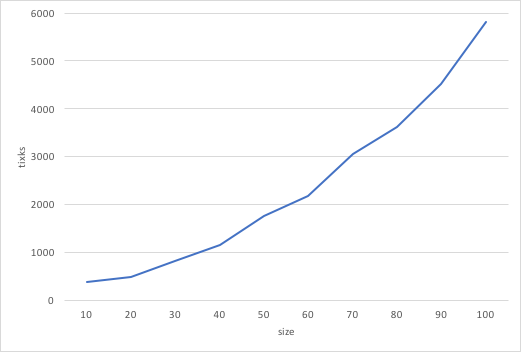
\includegraphics[width=0.8\textwidth]{ticks-size}
	\caption{Variação do tempo de exploração em função do tamanho do quadrado a explorar}
	\label{ticks-size}
\end{figure}

Os resultados obtidos podem ser observados no gráfico da Figura~\ref{ticks-size}, que sugere complexidade quadrática do nosso modelo em função do tamanho. Ora, isto faz imenso sentido uma vez que os \spotters têm que percorrer todo o tabuleiro e a sua área é igual ao quadrado do tamanho do lado.

Quando variamos o número de minérios, mantendo o tamanho constante a 30 e 5 agentes de cada tipo, deixam de ser os \spotters os últimos a terminar a exploração e passam a ser os \transporters. Isto é razoável, se pensarmos que com mais minérios para extrair, os \producers terão de continuar a extração mesmo depois de todos os \spotters terminarem de percorrer toda a área, pois terão acumulado os vários minérios a extrair nas suas filas. Já os \transporters, nunca podem terminar antes dos \producers, dado que terão de transportar o minério apenas depois de este ser extraído.

\begin{figure}[h]
	\centering
    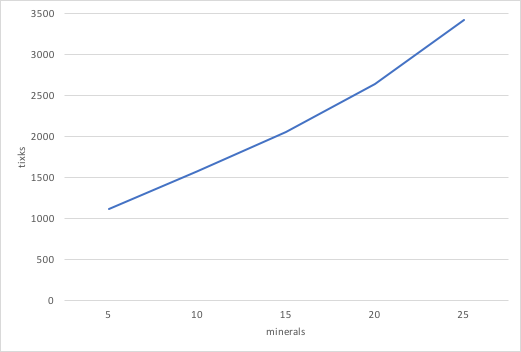
\includegraphics[width=0.8\textwidth]{ticks-minerals}
	\caption{Variação do tempo de exploração em função do número total de minérios}
	\label{ticks-minerals}
\end{figure}

Os resultados desta segunda experiência podem ser observados no gráfico da Figura~\ref{ticks-minerals}, que sugere complexidade linear do nosso modelo em função do número de minérios. Faz sentido que assim seja, dado que para extrair e transportar um mineral é gasto no máximo o tempo de ida e volta até lá mais o tempo de extração, que é igual à quantidade de minério, que por sua vez, apesar de não ser sempre igual, varia sempre entre os mesmos valores que mantivemos ao longo das experiências.

\subsection{Percentagem de utilização dos agentes}

%%%%%%%%%%%%%%
% CONCLUSOES %
%%%%%%%%%%%%%%
\chapter{Conclusões}

\section{Da análise dos resultados das experiências levadas a cabo}

\section{Do desenvolvimento do trabalho e aplicabilidade de SMA ao cenário proposto}

%%%%%%%%%%%%%%%%%
% MELHORAMENTOS %
%%%%%%%%%%%%%%%%%
\chapter{Melhoramentos}

\todonew[inline]{sugestões para melhoramentos a introduzir no programa}

Alguns possíveis melhoramentos ao nosso projeto são:

\begin{itemize}
	\item \Spotters decidirem entre si a divisão do espaço a explorar;
	\item Ao ser escolhido um \producer ou \transporter ter em conta o número de tarefas que estão a realizar de forma a maximizar o esforço dos mesmos;
	\item Ser possível de alterar o percurso dos agentes. Exemplo: Se ao atribuir a um \transporter uma tarefa e ficar em caminho ir a nave mãe descarregar, ele deveria descarregar e assim teria mais capacidade no final da tarefa;
	\item Atribuir os \transporters de forma eficiente tendo em conta a capacidade dos mesmos. Exemplo: Se um existe um \transporter que demora mais tempo mas tem capacidade para recolher o minério todo, deve ser selecionado em vez de atribuir pedaços de minério a vários \transporters que no final demorem mais tempo a recolher o minério todo;
\end{itemize}

%%%%%%%%%%%%
% RECURSOS %
%%%%%%%%%%%%
\chapter{Recursos}

\section{Bibliografia}

\begin{itemize}
	\item \href{https://paginas.fe.up.pt/~eol/AIAD/1617/trabalhos.html#T05}{Enunciado do trabalho}
	\item \href{https://paginas.fe.up.pt/~eol/AIAD/aiad1617.html}{Slides das aulas teóricas}
	\item \href{https://paginas.fe.up.pt/~eol/AIAD/aulas/jade_en.pdf}{Slides sobre \jade}
	\item \href{https://paginas.fe.up.pt/~eol/AIAD/aulas/REPAST_intro_hlc.pdf}{Slides sobre \repast}
	\item \href{https://web.fe.up.pt/~hlc/doku.php?id=sajas}{Página do \sajas}
	\item \href{https://web.fe.up.pt/~hlc/doku.php?id=massim2dev}{Página da ferramenta \massim}
\end{itemize}

\section{Software}

\begin{itemize}
	\item \href{http://jade.tilab.com}{\jade}
	\item \href{http://repast.sourceforge.net/repast_3/index.html}{\repast}
	\item \href{https://web.fe.up.pt/~hlc/doku.php?id=sajas}{\sajas}
\end{itemize}

\section{Elementos do grupo}
\todochange[inline]{indicar percentagem aproximada de trabalho efetivo de cada elementos do grupo}
\begin{itemize}
	\item Ângela Cardoso - \%
	\item Diogo Ferreira - \%
	\item Marina Camilo - \%
\end{itemize}


%%%%%%%%%%%%
% APENDICE %
%%%%%%%%%%%%
\chapter{Apêndice}

\todonew[inline]{manual do utilizador (sucinto)}

Após a criação de um projeto \java com o código entregue e adicionadas as bibliotecas de \sajas, \jade e \repast, é necessário correr o programa com a \texttt{Main class: main.Simulation}.

Ao correr, vai ser apresentado a consola do \repast. Começando a simulação será apresentada uma janela onde decorrerá a simulação idêntica a esta:

\begin{figure}[h]
	\centering
	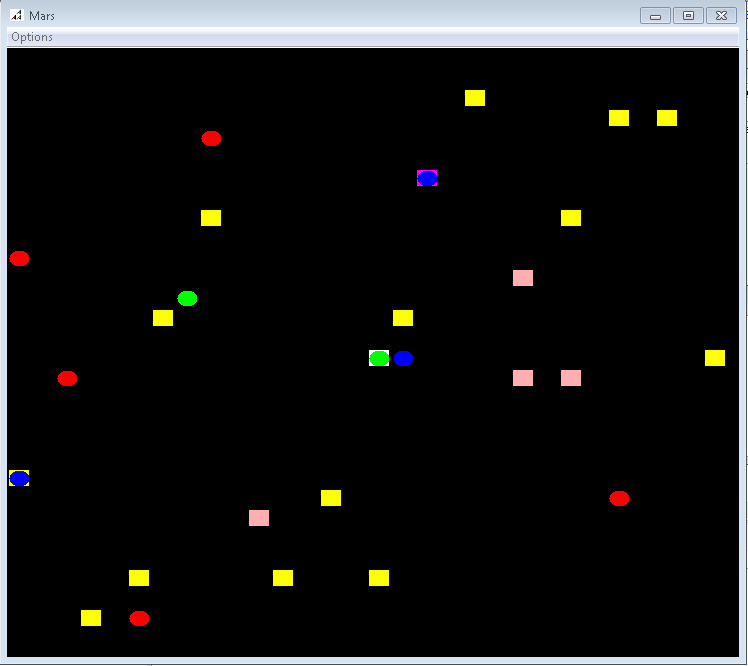
\includegraphics[width=0.8\textwidth]{simulacao}
	\caption{Exemplo de uma simulação}
	\label{simulacao}
\end{figure}

A simulação pode correr com diferentes tamanhos, números de minerais, \spotters, \producers, \transporters e a capacidade dos \transporters. Desta forma, também a  percentagem do mineral e o número de fragmentos encontrados num mineral podem ser alterados.
Assim, para alterar os parâmetros da simulação descritos acima é necessário aceder a classe \java \texttt{main.Environment}:

\begin{figure}[h]
	\centering
	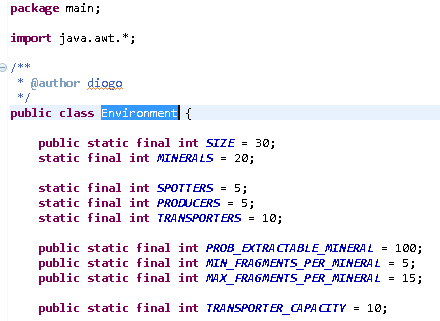
\includegraphics[width=0.8\textwidth]{javaEnvironment}
	\caption{Valores da Simulação}
	\label{javaEnvironment}
\end{figure}

\end{document}